% ============================================================================
% REQUIRED PACKAGES & CONFIGURATIONS FOR COMPILING THIS EXPERIMENT:
% ----------------------------------------------------------------------------
% \usepackage{circuitikz}      % For drawing op-amp circuit schematics
% \usepackage{pgfplots}        % For professional waveform and Bode plots
% \pgfplotsset{compat=1.18}    % Ensures modern rendering engine defaults
% \usepackage{booktabs}        % For publication-grade tables
% \usepackage{amsmath}         % For mathematical formulas
% \usepackage{siunitx}         % For standard scientific units
% ============================================================================

\chapter{Inverting and Non-Inverting Amplifiers Using Op-amps}

\section{Aim}
To design, set up, and analyze Operational Amplifier (Op-Amp) based Inverting and Non-Inverting Amplifiers using IC 741. The specific objectives are:
\begin{enumerate}
	\item To verify the closed-loop voltage gain for both inverting and non-inverting configurations.
	\item To observe and record the input-output phase relationship for each configuration.
	%\item To plot the frequency response curves and determine the $-3\text{ dB}$ bandwidth for both amplifiers.
\end{enumerate}

\section{Pre-Lab Assignment}
\begin{enumerate}[label=(\roman*)]
	\item Review the concept of the \emph{ideal op-amp} (infinite open-loop gain, infinite input impedance, zero output impedance) and the two golden rules of negative feedback analysis: (a) no current flows into the input terminals, and (b) the differential input voltage is zero (virtual short).
	\item For a given gain assigned to your batch, design suitable resistor values for both the inverting and non-inverting configurations.
	\item Simulate both designed circuits in LTspice (Pre-Lab~2) using the \texttt{OPAmp} or \texttt{UniversalOpAmp2} macro-model. Run a \texttt{.tran} analysis with a $1\,\text{kHz}$ sine input and verify the expected gain and phase (inverted/non-inverted) at the output.
	%\item Run a \texttt{.ac} analysis on the LTspice model and note the closed-loop bandwidth; compare this with the manufacturer's Gain-Bandwidth Product (GBW) specification for the IC 741 ($\approx 1\,\text{MHz}$) using the Gain-Bandwidth trade-off relation of Equation~\eqref{eq:gbw}.
\end{enumerate}

\section{Components and Equipment Required}
The required equipment and electronic components are listed in Table \ref{tab:components_opamp}.
\begin{table}[h!]
	\centering
	\begin{tabular}{@{}cll@{}}
		\toprule
		S.No. & Component/Equipment & Specification \\
		\midrule
		1  & Operational Amplifier IC & $\mu$A741 (or equivalent), 1 no. \\
		2  & Resistors & \SI{1}{\kilo\Omega}, \SI{10}{\kilo\Omega}, \SI{22}{\kilo\Omega} \\
		3  & Dual Regulated DC Power Supply & $\pm 15\,\text{V}$ \\
		4  & Function Generator & Sine wave, 1\,kHz\\
		5  & Digital Storage Oscilloscope & 2-channel, 20--50\,MHz bandwidth \\
		6  & Breadboard and connecting wires & -- \\
		\bottomrule
	\end{tabular}
	\caption{Components and equipment list.}
		\label{tab:components_opamp}
\end{table}

\section{Theory}

The operational amplifier (op-amp) is a high-gain DC-coupled voltage amplifier with differential inputs and single-ended output. When combined with an external negative feedback network, it realises a wide range of precise linear functions, the most fundamental being the inverting and non-inverting amplifiers. Analysis of both configurations proceeds from the \emph{ideal op-amp} assumptions:
\begin{enumerate}[label=(\alph*)]
	\item The input bias currents are zero (infinite input impedance), so no current flows into either input terminal.
	\item The open-loop gain $A_{OL}$ is infinite, so with negative feedback the differential input voltage $v_+ - v_- \to 0$ (the \emph{virtual short} condition).
\end{enumerate}
\subsection{Inverting Amplifier Configuration}
In the inverting amplifier, the input signal $v_{in}$ is applied to the inverting terminal (pin 2) through resistor $R_1$, while the non-inverting terminal (pin 3) is connected to ground through a bias-compensating resistor $R_{comp}$. Negative feedback is established via feedback resistor $R_f$.

Due to the extremely high open-loop gain and high input impedance of the op-amp, the differential voltage across the input terminals is virtually zero ($v_d \approx 0$). Consequently, the inverting input is held at a potential equal to the non-inverting terminal (0 V), creating a **Virtual Ground**.
\begin{equation}
	i_1 = \frac{v_{in} - 0}{R_1}, \quad i_f = \frac{0 - v_{out}}{R_f}
\end{equation}
Since no current enters the ideal op-amp terminal ($i_1 = i_f$):
\begin{equation}
	A_v = \frac{v_{out}}{v_{in}} = -\frac{R_f}{R_1}
\end{equation}
The negative sign indicates a $180^\circ$ phase shift between the input and output signals.

\subsection{Non-Inverting Amplifier Configuration}
In the non-inverting amplifier, the input signal $v_{in}$ is applied directly to the non-inverting terminal (pin 3). The feedback network ($R_1$ and $R_f$) forms a voltage divider that feeds a portion of the output voltage back to the inverting terminal (pin 2).

Applying the virtual short concept ($v_- = v_+ = v_{in}$):
\begin{equation}
	v_{in} = v_{out} \left( \frac{R_1}{R_1 + R_f} \right)
\end{equation}
Rearranging gives the closed-loop voltage gain:
\begin{equation}
	A_v = \frac{v_{out}}{v_{in}} = 1 + \frac{R_f}{R_1}
\end{equation}
The positive sign confirms that the output waveform is in phase ($0^\circ$ phase shift) with the input signal.

%\subsection{Gain--Bandwidth Trade-off}
%
%A practical op-amp has a finite, frequency-dependent open-loop gain that rolls off at $-20\,\text{dB/decade}$ beyond a low corner frequency, characterised by the Gain-Bandwidth Product (GBW), a constant for a given op-amp (e.g., $\approx 1\,\text{MHz}$ for the 741). For a closed-loop gain $A_{v}$, the resulting closed-loop bandwidth is approximately
%\begin{equation}
%	f_{closed\text{-}loop} \approx \frac{GBW}{|A_v|}\,.
%	\label{eq:gbw}
%\end{equation}
%Equation~\eqref{eq:gbw} shows that increasing the closed-loop gain (by increasing $R_f/R_1$) necessarily reduces the usable bandwidth of the amplifier -- a fundamental trade-off that will be verified experimentally in this experiment.


\section{Circuit Diagram}
The circuit schematics for both configurations are detailed in Figures \ref{fig:inv_circuit} and \ref{fig:noninv_circuit}.

\begin{figure}[h!]
	\centering
	\begin{circuitikz}[scale=0.9, line width=0.8pt, transform shape]
		% Op-amp
		\draw (0,0) node[op amp] (opamp) {LM 741};
		
		% Inverting path
		\draw (opamp.-) -- (-1.5, 0.5) to[R, l_=$R_1\ (\SI{1}{\kilo\Omega})$] (-3.5, 0.5) to[sV, l_=$v_{in}$] (-3.5, -2) node[ground] {};
		
		% Non-inverting path
		\draw (opamp.+) to[R, l_=$R_{comp}$] (-1.2, -2) node[ground] {};
		
		% Feedback loop
		\draw (opamp.-) -- (-1.2, 0.5) -- (-1.2, 1.8) to[R, l=$R_f\ (\SI{10}{\kilo\Omega})$] (1.5, 1.8) -- (1.5, 0) -- (opamp.out);
		
		% Output node
		\draw (opamp.out) -- (2.5, 0) node[right] {$v_{out}$};
		
		% Power supplies
		%\draw (opamp.up) -- (-0.04, 1.2) node[above] {$+V_{CC} = +15\text{ V}$};
		% Negative power line (goes straight down by 0.6 units)
		\draw (opamp.down) -- ++(0, -0.6) node[below] {$-15\text{ V}$};
		\draw (opamp.up) -- ++(0, 0.6) node[right] {$+15\text{ V}$};
		% Connection dots
		\node[circle, fill, inner sep=1.5pt] at (-1.2, 0.5) {};
		\node[circle, fill, inner sep=1.5pt] at (1.5, 0) {};
		%\node[circle, fill, inner sep=1.5pt] at (-0.1, -1.2) {};
		% Pin numbers attached to terminal anchors
		\node[font=\small, above right] at (opamp.-) {2};   % Inverting Input
		\node[font=\small, above right] at (opamp.+) {3};   % Non-Inverting Input
		\node[font=\small, above left]  at (opamp.out) {6}; % Output
		\node[font=\small, above right] at (opamp.up) {7};  % +VCC
		\node[font=\small, below right] at (opamp.down) {4};% -VEE
	\end{circuitikz}
	\caption{Inverting Amplifier Circuit Diagram}
	\label{fig:inv_circuit}
\end{figure}

\begin{figure}[h!]
	\centering
	\begin{circuitikz}[scale=0.9, line width=0.8pt, transform shape]
		% Op-amp
		\draw (0,0) node[op amp] (opamp) {LM 741};
		
		% Inverting path
		\draw (opamp.-) -- (-1.5, 0.5) to[R, l_=$R_1\ (\SI{1}{\kilo\Omega})$] (-3.5, 0.5) to (-3.5, -2) node[ground] {};
		 
		% Non-inverting path
		\draw (opamp.+) to[sV, l_=$v_{in}$] (-1.2, -2) node[ground] {};
		
		% Feedback loop
		\draw (opamp.-) -- (-1.2, 0.5) -- (-1.2, 1.8) to[R, l=$R_f\ (\SI{10}{\kilo\Omega})$] (1.5, 1.8) -- (1.5, 0) -- (opamp.out);
		
		% Output node
		\draw (opamp.out) -- (2.5, 0) node[right] {$v_{out}$};
		
		% Power supplies
		%\draw (opamp.up) -- (-0.04, 1.2) node[above] {$+V_{CC} = +15\text{ V}$};
		% Negative power line (goes straight down by 0.6 units)
		\draw (opamp.down) -- ++(0, -0.6) node[below] {$-15\text{ V}$};
		\draw (opamp.up) -- ++(0, 0.6) node[right] {$+15\text{ V}$};
		% Connection dots
		\node[circle, fill, inner sep=1.5pt] at (-1.2, 0.5) {};
		\node[circle, fill, inner sep=1.5pt] at (1.5, 0) {};
		%\node[circle, fill, inner sep=1.5pt] at (-0.1, -1.2) {};
		% Pin numbers attached to terminal anchors
		\node[font=\small, above right] at (opamp.-) {2};   % Inverting Input
		\node[font=\small, above right] at (opamp.+) {3};   % Non-Inverting Input
		\node[font=\small, above left]  at (opamp.out) {6}; % Output
		\node[font=\small, above right] at (opamp.up) {7};  % +VCC
		\node[font=\small, below right] at (opamp.down) {4};% -VEE
	\end{circuitikz}
	\caption{Non-Inverting Amplifier Circuit Diagram}
	\label{fig:noninv_circuit}
\end{figure}

\section{Design}
\subsection{Inverting Amplifier Design ($|A_v| = 10$)}
\begin{enumerate}
	\item Choose an input resistor $R_1 = \SI{1}{\kilo\Omega}$ to ensure negligible loading on the input signal source while keeping currents within normal limits.
	\item Calculate the feedback resistor $R_f$:
	
	We know that the gain 
	\[ 
	A_v=-\frac{R_f}{R_1}
	\]
	\begin{equation}
		|A_v| = \frac{R_f}{R_1} \implies 10 = \frac{R_f}{\SI{1}{\kilo\Omega}} \implies R_f = \SI{10}{\kilo\Omega}
	\end{equation}
	\item Calculate the offset-minimizing resistor $R_{comp}$ connected to the non-inverting terminal to balance input bias currents:
	\begin{equation}
		R_{comp} = R_1 \parallel R_f = \frac{1\text{ k}\Omega \cdot 10\text{ k}\Omega}{1\text{ k}\Omega + 10\text{ k}\Omega} \approx \SI{909}{\Omega} \quad (\text{Select standard value: } \SI{1}{\kilo\Omega})
	\end{equation}
\end{enumerate}

\subsection{Non-Inverting Amplifier Design ($A_v = 11$)}
\begin{enumerate}
	\item Select $R_1 = \SI{1}{\kilo\Omega}$.
	\item Determine $R_f$:
	\begin{equation}
		A_v = 1 + \frac{R_f}{R_1} \implies 11 = 1 + \frac{R_f}{\SI{1}{\kilo\Omega}} \implies R_f = \SI{10}{\kilo\Omega}
	\end{equation}
\end{enumerate}

\section{Procedure}
\subsection{Inverting Amplifier Setup and Measurement}
\begin{enumerate}
	\item Connect $+15\text{ V}$ DC to pin 7 ($+V_{CC}$) and $-15\text{ V}$ DC to pin 4 ($-V_{EE}$) of IC 741 on the breadboard.
	\item Construct the inverting amplifier circuit shown in Figure \ref{fig:inv_circuit} with $R_1 = \SI{1}{\kilo\Omega}$ and $R_f = \SI{10}{\kilo\Omega}$.
	\item Connect Channel 1 of the DSO across the input $v_{in}$ and Channel 2 across the output $v_{out}$.
	\item Set the function generator to produce a sine wave of $1.0\text{ V}_{p-p}$ at a frequency of \SI{1}{\kilo\hertz}.
	\item Measure the peak-to-peak output voltage $V_{out}$ and observe the phase relation between $v_{in}$ and $v_{out}$.
%	\item Keep $V_{in}$ constant at $1.0\text{ V}_{p-p}$ and vary the input frequency from \SI{10}{\hertz} to \SI{1}{\mega\hertz}. Log $V_{out}$ at each frequency step in Table \ref{tab:obs_freq}.
\end{enumerate}

\subsection{Non-Inverting Amplifier Setup and Measurement}
\begin{enumerate}
	\item Reconfigure the circuit to form the non-inverting amplifier as shown in Figure \ref{fig:noninv_circuit}.
	\item Apply a $1.0\text{ V}_{p-p}$ sine wave at \SI{1}{\kilo\hertz} to the non-inverting input terminal (pin 3).
	\item Measure $V_{out}$ and observe the phase shift relative to $v_{in}$.
%	\item Sweep the frequency from \SI{10}{\hertz} to \SI{1}{\mega\hertz} while maintaining $V_{in} = 1.0\text{ V}_{p-p}$ and record the output amplitude.
\end{enumerate}

\section{Precautions}
\begin{enumerate}
	\item Do not exceed the maximum supply voltage limits ($\pm 18\text{ V}$) for IC 741.
	\item Reversed supply connections can permanently damage the IC.
	\item Before applying input signal to the IC, power the IC.
	\item Always establish a common ground connection between the power supply, signal generator, and oscilloscope.
	\item To avoid saturation distortion, ensure that $V_{in} \cdot A_v$ does not exceed the op-amp saturation limits ($\approx \pm 13\text{ V}$).
	\item Switch off the power supply before changing any circuit connections.
\end{enumerate}

\section{Model Graph / Expected Waveforms}
Figure \ref{fig:wave_inv} and \ref{fig:wave_noninv}  shows the expected input-output waveforms illustrating the phase shifts for both configurations. %Figure \ref{fig:model_bode} shows the expected frequency response.

%\begin{figure}[h!]
%	\centering
%	\begin{tikzpicture}
%		\begin{axis}[
%			axis lines=middle,
%			xlabel={$t\text{ (ms)}$},
%			ylabel={Voltage (V)},
%			xmin=0, xmax=2,
%			ymin=-12, ymax=12,
%			grid=both,
%			grid style={line width=.1pt, draw=gray!20},
%			major grid style={line width=.2pt, draw=gray!40},
%			width=11cm, height=5.5cm,
%			title={\textbf{Expected Time-Domain Waveforms (Inverting vs Non-Inverting)}},
%			legend pos=outer north east
%			]
%			% Input Signal
%			\addplot[thick, black, domain=0:2, samples=100] {1*sin(deg(2*pi*x))};
%			\addlegendentry{$v_{in}\ (1\text{ V}_{p-p})$}
%			
%			% Inverting Output
%			\addplot[thick, blue, dashed, domain=0:2, samples=100] {-10*sin(deg(2*pi*x))};
%			\addlegendentry{$v_{out}$ (Inverting, $A_v=-10$)}
%			
%			% Non-Inverting Output
%			\addplot[thick, red, dotted, domain=0:2, samples=100] {11*sin(deg(2*pi*x))};
%			\addlegendentry{$v_{out}$ (Non-Inv, $A_v=+11$)}
%		\end{axis}
%	\end{tikzpicture}
%	\caption{Model Input and Output Waveforms at \SI{1}{\kilo\hertz}}
%	\label{fig:model_waveforms}
%\end{figure}

\begin{figure}[h!]
	\centering
	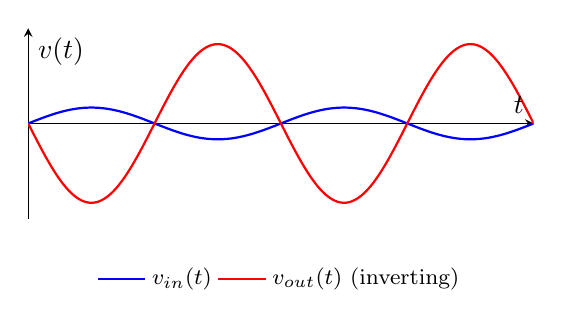
\begin{tikzpicture}
		\begin{axis}[
			width=8cm, height=4cm,
			xlabel={$t$}, ylabel={$v(t)$},
			axis lines=middle,
			ymin=-6, ymax=6,
			xtick=\empty, ytick=\empty,
			domain=0:2, samples=200,
			legend style={draw=none, font=\footnotesize, at={(0.5,-0.2)}, anchor=north, legend columns=2}
			]
			\addplot[blue, thick] {sin(360*x)};
			\addlegendentry{$v_{in}(t)$}
			\addplot[red, thick] {-5*sin(360*x)};
			\addlegendentry{$v_{out}(t)$ (inverting)}
		\end{axis}
	\end{tikzpicture}
	\caption{Expected waveforms for the inverting amplifier: $v_{out}$ is amplified and $180^\circ$ out of phase with $v_{in}$.}
	\label{fig:wave_inv}
\end{figure}

\begin{figure}[h!]
	\centering
	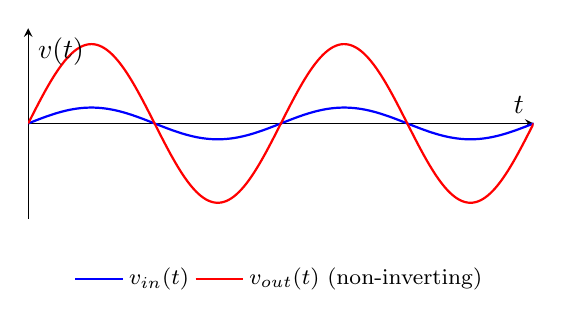
\begin{tikzpicture}
		\begin{axis}[
			width=8cm, height=4cm,
			xlabel={$t$}, ylabel={$v(t)$},
			axis lines=middle,
			ymin=-6, ymax=6,
			xtick=\empty, ytick=\empty,
			domain=0:2, samples=200,
			legend style={draw=none, font=\footnotesize, at={(0.5,-0.2)}, anchor=north, legend columns=2}
			]
			\addplot[blue, thick] {sin(360*x)};
			\addlegendentry{$v_{in}(t)$}
			\addplot[red, thick] {5*sin(360*x)};
			\addlegendentry{$v_{out}(t)$ (non-inverting)}
		\end{axis}
	\end{tikzpicture}
	\caption{Expected waveforms for the non-inverting amplifier: $v_{out}$ is amplified and in phase with $v_{in}$.}
	\label{fig:wave_noninv}
\end{figure}
%\begin{figure}[h!]
%	\centering
%	\begin{tikzpicture}
%		\begin{axis}[
%			width=9cm, height=5cm,
%			xlabel={Frequency $f$ (Hz, log scale)},
%			ylabel={Closed-loop Gain (dB)},
%			xmode=log,
%			xmin=10, xmax=1e7,
%			ymin=0, ymax=60,
%			grid=both,
%			axis lines=left,
%			legend style={draw=none, font=\footnotesize, at={(0.5,-0.2)}, anchor=north, legend columns=1}
%			]
%			\addplot[blue, thick, domain=10:1e7, samples=300] {20*log10( 1000 / sqrt(1+(x/1000)^2) )};
%			\addlegendentry{$A_v = 60\,\text{dB}$ (higher gain, lower BW)}
%			\addplot[red, thick, domain=10:1e7, samples=300] {20*log10( 20 / sqrt(1+(x/50000)^2) )};
%			\addlegendentry{$A_v = 26\,\text{dB}$ (lower gain, higher BW)}
%		\end{axis}
%	\end{tikzpicture}
%	\caption{Illustration of the Gain--Bandwidth trade-off (Equation~\eqref{eq:gbw}): higher closed-loop gain results in a proportionally lower closed-loop bandwidth, for a fixed op-amp GBW.}
%	\label{fig:gbw_tradeoff}
%\end{figure}


%\section{Observation Tables}
%\begin{table}[h!]
%	\centering
%	\begin{tabular}{@{}ccccc@{}}
%		\toprule
%		Frequency $f$ (Hz) & $V_{in,pp}$ (V) & $V_{out,pp}$ (V) & $A_v$ & $A_v$ (dB) \\
%		\midrule
%		&  &  &  &  \\
%		&  &  &  &  \\
%		&  &  &  &  \\
%		&  &  &  &  \\
%		&  &  &  &  \\
%		\bottomrule
%	\end{tabular}
%	\caption{Frequency response data for the inverting amplifier (repeat a similar table for the non-inverting amplifier).}
%	\label{tab:expt3_freq_obs}
%\end{table}
%
%\begin{table}[h!]
%	\centering
%	\begin{tabular}{@{}lcccc@{}}
%		\toprule
%		Configuration & $A_v$ (theory) & $A_v$ (measured) & $f_{-3dB}$ (theory) & $f_{-3dB}$ (measured) \\
%		\midrule
%		Inverting amplifier &  &  &  &  \\
%		Non-inverting amplifier &  &  &  &  \\
%		\bottomrule
%	\end{tabular}
%	\caption{Summary: theoretical vs. measured gain and bandwidth.}
%	\label{tab:expt3_summary}
%\end{table}

\section{Result}
The performance metrics of the Op-Amp Inverting and Non-Inverting Amplifiers were experimentally measured and analyzed:

\section{Questions}
\begin{enumerate}
	\item What is meant by a "Virtual Ground" in op-amp circuits, and why does it not exist at the inverting pin of a non-inverting amplifier?
	\item Why does a non-inverting amplifier exhibit a significantly higher input impedance than an inverting amplifier?
	\item What happens to the output waveform if the input amplitude is increased such that $V_{in} \cdot A_v > V_{sat}$?
	\item Explain how the Gain-Bandwidth Product (GBWP) limits the maximum operational frequency of an op-amp circuit when closed-loop gain is increased.
	\item What is the function of the offset-nulling pins (pins 1 and 5) on the IC 741 operational amplifier?
\end{enumerate}